\documentclass[14pt]{beamer}

% beamer definieert 'definition' al, maar dan engels :(
% fix van:
% http://tex.stackexchange.com/questions/38392/how-to-rename-theorem-or-lemma-in-beamer-to-another-language
\usepackage[dutch]{babel}
\uselanguage{dutch}
\languagepath{dutch}
\deftranslation[to=dutch]{Definition}{Definitie}

\usepackage{array}

\usepackage{graphicx}
\usepackage{float}
\usepackage{amssymb}
\usepackage{color}
\usepackage{listings}

\newcommand{\id}{\text{id}}
\newcommand{\N}{\mathbb{N}}
\newcommand{\Z}{\mathbb{Z}}
\newcommand{\R}{\mathbb{R}}
\newcommand{\cat}[1]{\mathbf{#1}}
\newcommand{\Ch}[1]{\mathbf{Ch}(#1)}
\newcommand{\Hom}[3]{\mathbf{Hom}_{#1}(#2, #3)}

\newcommand{\iso}{\cong}
\newcommand{\tot}[1]{\xrightarrow{\,\,{#1}\,\,}}
\newcommand{\eps}{\varepsilon}
\newcommand{\I}{\,\mid\,}
\newcommand{\then}{\Rightarrow}
\newcommand{\inject}{\hookrightarrow}
\newcommand{\del}{\partial}
\newcommand{\nsubgrp}{\trianglelefteq}

% relative to the one who includes us :(
\graphicspath{ {../images/} }

\newcommand{\todo}[1]{
	\addcontentsline{tdo}{todo}{\protect{#1}}
	$\ast$ \marginpar{\tiny $\ast$ #1}
}
\makeatletter
	\newcommand \listoftodos{\section*{Todo list} \@starttoc{tdo}}
	\newcommand\l@todo[2]{
		\par\noindent \textit{#2}, \parbox{10cm}{#1}\par
	}
\makeatother


\title{Dold-Kan correspondentie
	\huge $$ \Ch{\cat{Ab}} \simeq \cat{sAb} $$}
\author{Joshua Moerman}
\institute[Radboud Universiteit Nijmegen]{Begeleid door Moritz Groth}
\date{}

\begin{document}


\begin{frame}
	\titlepage
\end{frame}


\begin{frame}
	\frametitle{Wat is $\Ch{\cat{Ab}}$?}
	\begin{definition}
	Een \emph{ketencomplex} $C$ bestaat uit abelse groepen met groepshomomorfisme:
	$$ \cdots \to C_4 \tot{\del_3} C_3 \tot{\del_2} C_2 \tot{\del_1} C_1 \tot{\del_0} C_0 $$

	zodat $\del_n \circ \del_{n+1} = 0$ voor alle $n \in \N$.
	\end{definition}
\end{frame}


\begin{frame}
	\frametitle{Voorbeeld}
	\centering \vspace{-0.5cm}
	Bekijk $\Delta^n \tot{f} X$,\, dwz...\, \raisebox{-.2\height}{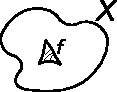
\includegraphics{simplex_in_X}}
	\bigskip
	\bigskip

	\includegraphics<1>{singular_chaincomplex1}
	\includegraphics<2>{singular_chaincomplex2}
	\includegraphics<3>{singular_chaincomplex3}
\end{frame}


\begin{frame}
	\frametitle{Interessant?}
	Gegeven een ketencomplex $C$:
	$$ \cdots \to C_4 \tot{\del_3} C_3 \tot{\del_2} C_2 \tot{\del_1} C_1 \tot{\del_0} C_0 $$
	met $\del_n \circ \del_{n+1} = 0$
	\bigskip
	
	Dan geldt $im(\del_{n+1}) \trianglelefteq ker(\del_n)$

	Definieer: $H_n(C) = ker(\del_{n-1}) / im(\del_n)$

	(met $ker(\del_0) = C_0$ per conventie)
\end{frame}


\begin{frame}
	\frametitle{Voorbeeld}
	$ \cdots \to C_1 \tot{\del_0} C_0 $, wat is $ H_1 = \frac{ker(\del_0)}{im(\del_1)} $?
	\bigskip

	\begin{tabular}{m{0.3\textwidth} m{0.7\textwidth}}
		\includegraphics<1>{singular_homology1}
		\includegraphics<2->{singular_homology2}
		&
		$ \sigma_1 - \sigma_2 + \sigma_3 \in ker (\del_0) $ \newline
		\visible<2->{
		$ \del_1(\tau) = \sigma_1 - \sigma_2 + \sigma_3 $ \newline
		Dus $ \sigma_1 + \sigma_2 - \sigma_3 \in im (\del_1) $ \newline
		Dus $ 0 = [\sigma_1 - \sigma_2 + \sigma_3] \in H_1 $}
	\end{tabular}
	\bigskip

	\visible<3->{
	\begin{tabular}{m{0.3\textwidth} m{0.7\textwidth}}
		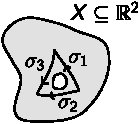
\includegraphics{singular_homology3}
		&
		$ \sigma_1 - \sigma_2 + \sigma_3 \in ker (\del_0) $ \newline
		Maar $ \sigma_1 - \sigma_2 + \sigma_3 \not \in im (\del_1) $ \newline
		Dus $ 0 \neq [\sigma_1 - \sigma_2 + \sigma_3] \in H_1 $
	\end{tabular}
	}

\end{frame}


\begin{frame}
	\frametitle{Dold-Kan Correspondentie}
	\begin{center}
	{\Large $ \Ch{\cat{Ab}} \simeq \cat{sAb} $}

	verder:
	{\Large $$ H_n(N(X)) \iso \pi_n(X) $$}
	waarbij $N : \cat{sAb} \tot{\simeq} \Ch{\cat{Ab}}$.
	\end{center}
\end{frame}


\begin{frame}
	\begin{center}
	\Huge Vragen?
	\end{center}
\end{frame}


\end{document}
